% Options for packages loaded elsewhere
\PassOptionsToPackage{unicode}{hyperref}
\PassOptionsToPackage{hyphens}{url}
\documentclass[
]{article}
\usepackage{xcolor}
\usepackage[margin=1in]{geometry}
\usepackage{amsmath,amssymb}
\setcounter{secnumdepth}{-\maxdimen} % remove section numbering
\usepackage{iftex}
\ifPDFTeX
  \usepackage[T1]{fontenc}
  \usepackage[utf8]{inputenc}
  \usepackage{textcomp} % provide euro and other symbols
\else % if luatex or xetex
  \usepackage{unicode-math} % this also loads fontspec
  \defaultfontfeatures{Scale=MatchLowercase}
  \defaultfontfeatures[\rmfamily]{Ligatures=TeX,Scale=1}
\fi
\usepackage{lmodern}
\ifPDFTeX\else
  % xetex/luatex font selection
\fi
% Use upquote if available, for straight quotes in verbatim environments
\IfFileExists{upquote.sty}{\usepackage{upquote}}{}
\IfFileExists{microtype.sty}{% use microtype if available
  \usepackage[]{microtype}
  \UseMicrotypeSet[protrusion]{basicmath} % disable protrusion for tt fonts
}{}
\makeatletter
\@ifundefined{KOMAClassName}{% if non-KOMA class
  \IfFileExists{parskip.sty}{%
    \usepackage{parskip}
  }{% else
    \setlength{\parindent}{0pt}
    \setlength{\parskip}{6pt plus 2pt minus 1pt}}
}{% if KOMA class
  \KOMAoptions{parskip=half}}
\makeatother
\usepackage{longtable,booktabs,array}
\usepackage{caption}
\captionsetup[table]{skip=6pt}
\newcounter{none} % for unnumbered tables
\usepackage{calc} % for calculating minipage widths
% Correct order of tables after \paragraph or \subparagraph
\usepackage{etoolbox}
\makeatletter
\patchcmd\longtable{\par}{\if@noskipsec\mbox{}\fi\par}{}{}
\makeatother
% Allow footnotes in longtable head/foot
\IfFileExists{footnotehyper.sty}{\usepackage{footnotehyper}}{\usepackage{footnote}}
\makesavenoteenv{longtable}
\usepackage{graphicx}
\makeatletter
\newsavebox\pandoc@box
\newcommand*\pandocbounded[1]{% scales image to fit in text height/width
  \sbox\pandoc@box{#1}%
  \Gscale@div\@tempa{\textheight}{\dimexpr\ht\pandoc@box+\dp\pandoc@box\relax}%
  \Gscale@div\@tempb{\linewidth}{\wd\pandoc@box}%
  \ifdim\@tempb\p@<\@tempa\p@\let\@tempa\@tempb\fi% select the smaller of both
  \ifdim\@tempa\p@<\p@\scalebox{\@tempa}{\usebox\pandoc@box}%
  \else\usebox{\pandoc@box}%
  \fi%
}
% Set default figure placement to htbp
\def\fps@figure{htbp}
\makeatother
\setlength{\emergencystretch}{3em} % prevent overfull lines
\providecommand{\tightlist}{%
  \setlength{\itemsep}{0pt}\setlength{\parskip}{0pt}}
\usepackage{bookmark}
\IfFileExists{xurl.sty}{\usepackage{xurl}}{} % add URL line breaks if available
\urlstyle{same}
% fallback for those not using the hyperref driver hyperxmp:
\makeatletter
\@ifundefined{xmpquote}{\newcommand{\xmpquote}[1]{#1}}{}
\makeatother
\hypersetup{
  hidelinks,
  pdfcreator={LaTeX via pandoc}}

\author{}
\date{}

\begin{document}

\section{BharatTrip Refund Escalations: Business Case \& Solution Proposal}\label{bharattrip-refund-escalations-business-case-solution-proposal}

\begin{quote}
\textbf{Executive Summary (TL;DR)}\\
BharatTrip is experiencing a spike in customer/agent refund escalations despite stable refund volumes. Our analysis identified a severe operational disconnect between Support and Finance, leading to \textbf{100 dropped tickets} and \textbf{149 short payments}. By implementing a \textbf{Single Source of Truth (SSOT)} and an \textbf{AI-Driven Data Reconciliation Workflow}, we deploy a "Digital Workforce." This allows existing teams to eliminate manual data leakage and automate agent communications, driving a projected \textbf{85\%+ drop in escalations} over the next quarter \textbf{without adding a single headcount}.
\end{quote}

\begin{center}\rule{0.5\linewidth}{0.5pt}\end{center}

\subsection{1. Defining the Problem}\label{defining-the-problem}

Customer and agent escalations regarding refunds are rising. The core underlying problem is a \textbf{severe operational disconnect between the Support and Finance teams}, characterized by siloed tracking systems and inconsistent definitions of refund statuses.

\subsubsection{Key Communication Failures:}\label{key-communication-failures}

\begin{enumerate}
\def\labelenumi{\arabic{enumi}.}
\tightlist
\item
  \textbf{Data Leakage}: Informal requests via WhatsApp and Email bypass the tracker altogether, meaning they are never reviewed or processed.
\item
  \textbf{``Closed'' Status Ambiguity}: The Support team marks tickets as ``Closed'' once handed off to Finance, misleading the agent into believing the refund has been disbursed.
\item
  \textbf{Hidden Policy Deductions}: Finance applies necessary deductions (e.g., cancellation fees) and processes payouts, but this information is never relayed back to the agent by Support, causing ``short payment'' escalations.
\end{enumerate}

\begin{center}\rule{0.5\linewidth}{0.5pt}\end{center}

\subsection{2. Data Analysis \& Insights}\label{data-analysis-insights}

By cross-referencing the \texttt{Support\_Tracker}, \texttt{Finance\_Tracker}, and \texttt{Escalations} logs via a deep database join, we identified the specific patterns driving the \textbf{155 total escalations}.

\begin{figure}[htbp]
    \centering
    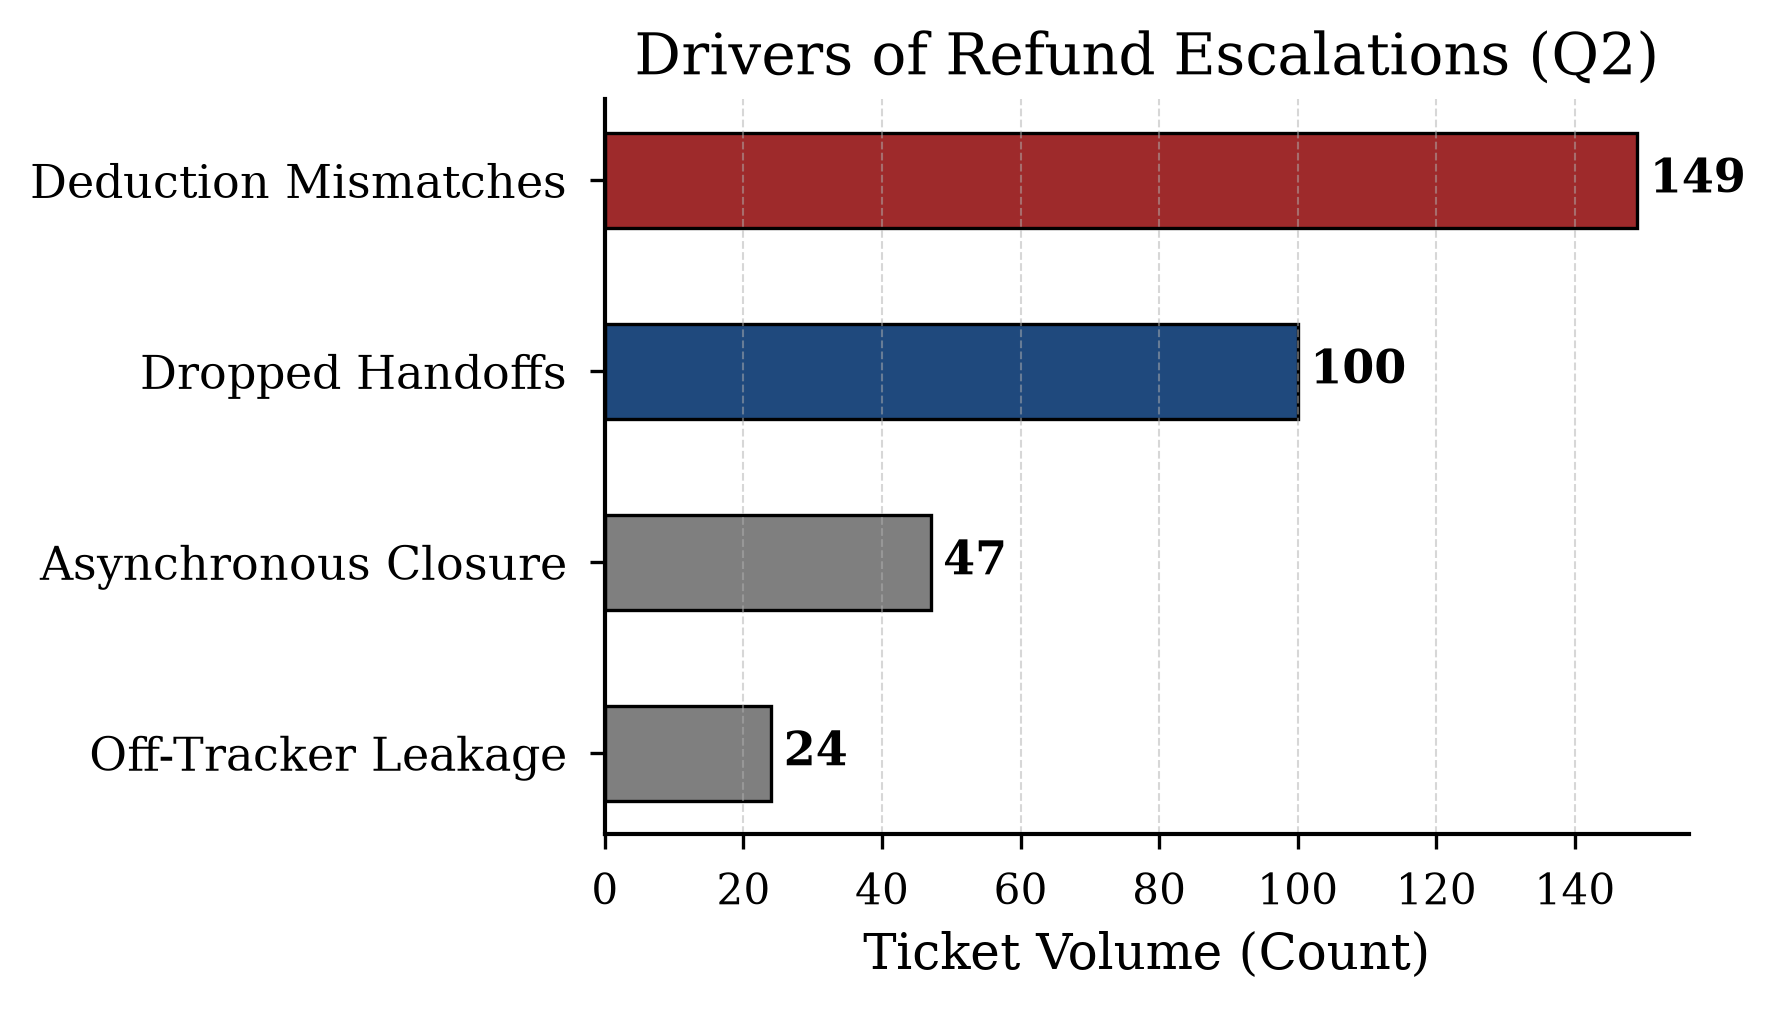
\includegraphics[width=\textwidth]{metrics.png}
    \caption{Visual breakdown of current support processing inefficiencies highlighting the 100 dropped handoffs and 149 mismatches.}
\end{figure}

\subsubsection{The Discrepancy Breakdown}\label{the-discrepancy-breakdown}

{\def\LTcaptype{none} % do not increment counter
\begin{longtable}[]{@{}
  >{\raggedright\arraybackslash}p{(\linewidth - 4\tabcolsep) * \real{0.3333}}
  >{\raggedright\arraybackslash}p{(\linewidth - 4\tabcolsep) * \real{0.3333}}
  >{\raggedright\arraybackslash}p{(\linewidth - 4\tabcolsep) * \real{0.3333}}@{}}
\toprule\noalign{}
\begin{minipage}[b]{\linewidth}\raggedright
Escalation Driver
\end{minipage} & \begin{minipage}[b]{\linewidth}\raggedright
Ticket Volume
\end{minipage} & \begin{minipage}[b]{\linewidth}\raggedright
Description
\end{minipage} \\
\midrule\noalign{}
\endhead
\bottomrule\noalign{}
\endlastfoot
\textbf{Dropped Handoffs} & \textbf{100} & Logged by Support, but entirely missing from Finance tracking. \\
\textbf{Deduction Mismatches} & \textbf{149} & Amount promised by Support differs from amount disbursed by Finance. \\
\textbf{Off-Tracker Leakage} & \textbf{24} & Escalations with ``no ref'' originating from unlogged WhatsApp/Email. \\
\textbf{Asynchronous Closure} & \textbf{47} & Processed by Finance but missing from Support. \\
\end{longtable}
}

\begin{quote}
\textbf{Insight:} While a naive net volume calculation (755 Support - 689 Finance) suggests only 66 missing tickets, our deep ID-to-ID database reconciliation reveals the true scale of the failure is \textbf{100 dropped tickets}, masked by duplicate records and asynchronous closures.
\end{quote}

\begin{center}\rule{0.5\linewidth}{0.5pt}\end{center}

\subsection{3. Designing a Zero-Headcount Solution}\label{designing-a-zero-headcount-solution}

To permanently bring escalations down without adding headcount, BharatTrip must establish a unified \textbf{Single Source of Truth (SSOT)} and redesign the workflow.

\subsubsection{The Single Source of Truth}\label{the-single-source-of-truth}
The SSOT is a centralized database that completely replaces the individual Support and Finance Excel trackers. The two teams stay in sync by operating off the exact same rows in real-time through a shared web portal. When Finance applies a payout deduction, the SSOT updates immediately, ensuring Support always sees the true financial status of the ticket before communicating with the agent.

\subsubsection{Trade-Offs: Automation vs. Manual Verification}\label{trade-offs-automation-vs-manual}
Given the compliance risks associated with financial payouts, we cannot automate the entire pipeline. We must strike a deliberate balance:
\begin{itemize}
\tightlist
\item \textbf{Automate (Data Ingestion):} We deploy an AI Agent to parse messy, unstructured WhatsApp and Email requests into structured SSOT rows. \textit{Why?} This is high-volume, low-risk administrative work. Automating it entirely eliminates the 24 "Off-Tracker Leaks."
\item \textbf{Automate (Reconciliation Detection):} The system automatically flags when Finance payouts are lower than Support quotes. \textit{Why?} Math is deterministic; automation catches the 149 mismatches instantly without human error.
\item \textbf{Deliberately Keep Manual (Approval \& Payout):} The AI is only permitted to \textit{draft} the explanatory emails explaining the short-payments to the agents. A human operator must review the AI's draft and click "Approve \& Send". Furthermore, the actual financial disbursement remains strictly manual. \textit{Why?} AI hallucinations in customer communication or automated banking APIs pose severe reputational and compliance risks. A Human-in-the-Loop (HITL) architecture ensures strict accountability.
\end{itemize}

\begin{center}\rule{0.5\linewidth}{0.5pt}\end{center}

\subsection{4. The AI Prototype: Enterprise-Ready Architecture}\label{the-ai-prototype-advanced-multi-agent-architecture}

To deliver a production-ready solution, I developed a \textbf{Streamlit Web Application} showcasing an advanced Multi-Agent architecture powered by \texttt{gemini-3.5-flash}. Rather than building a simple LLM script, I engineered a secure, deployable enterprise tool.

\begin{figure}[htbp]
    \centering
    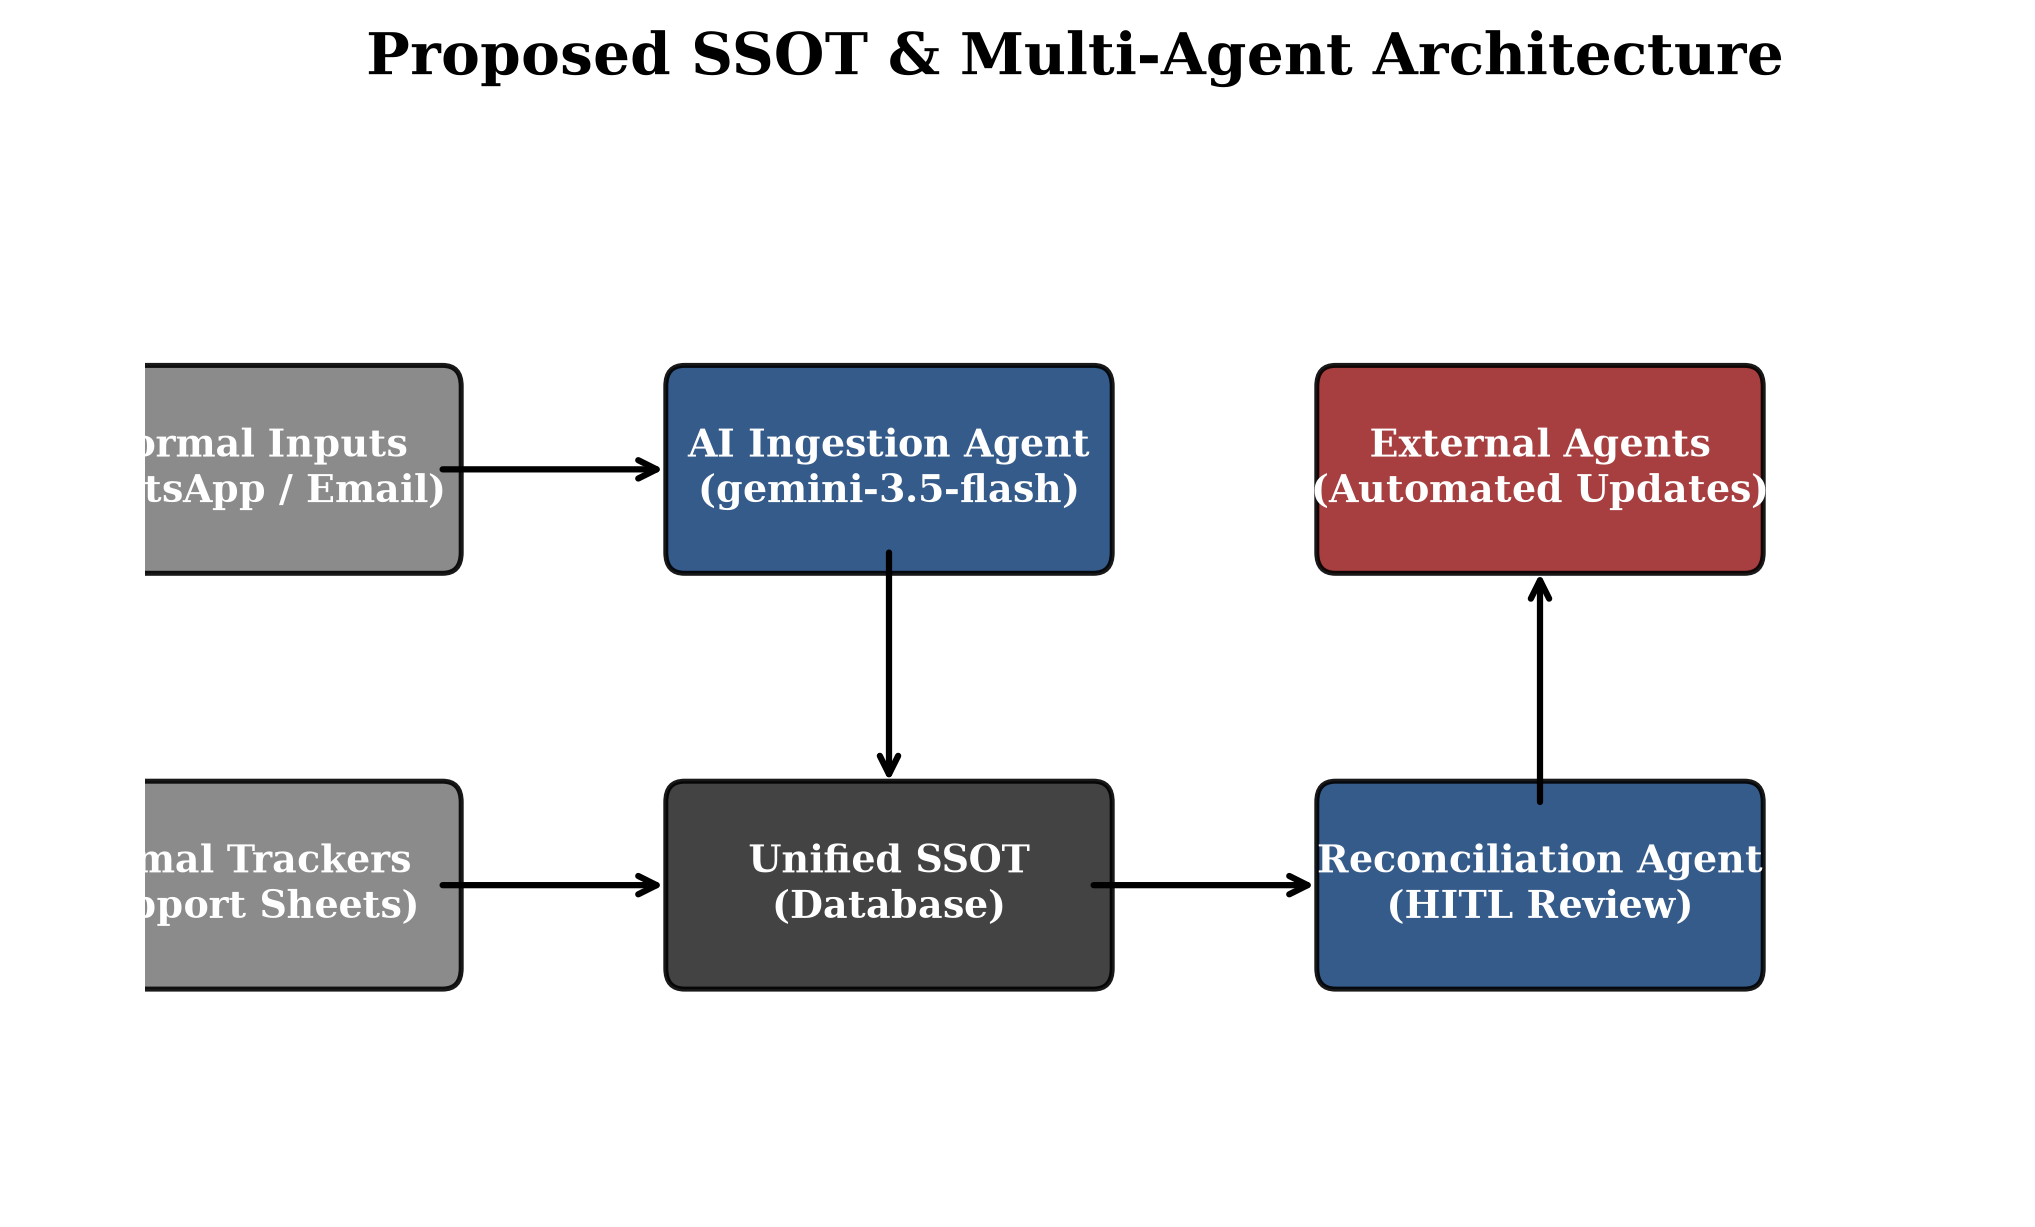
\includegraphics[width=\textwidth]{architecture.png}
    \caption{Proposed Multi-Agent System Architecture Flowchart}
\end{figure}

\subsubsection{Key Enterprise Features \& Security Mitigations}\label{operational-safety-risks-mitigations}
Deploying AI in financial workflows carries inherent risks (e.g., hallucinated refund amounts, unauthorized access, or PII leaks). Our architecture mitigates this using a \textbf{Defense-in-Depth} approach:
\begin{itemize}
\tightlist
\item \textbf{Identity Gateway \& RBAC}: The application enforces dual-role authorization. Managers have full access, while Operators are restricted.
\item \textbf{Data Privacy (PII Redaction)}: Sensitive identifiers in unstructured messages are automatically redacted via RegEx prior to ingestion. Furthermore, Operator roles see dynamically masked UI views.
\item \textbf{Data Loss Prevention (DLP)}: UI-level CSS injection prevents text selection and copying of sensitive fields.
\item \textbf{AI Confidence Guardrails}: The ingestion agent scores its own extractions and flags low-confidence data for mandatory human review.
\item \textbf{Human-In-The-Loop (HITL) \& Auditability}: The AI is strictly limited to \textit{drafting} emails and structuring data. A human must click "Approve \& Send", and every action is logged to a secure CSV for financial compliance.
\item \textbf{Unified Database Explorer}: A global search interface completely breaks down the silos between Support and Finance, serving as the ultimate Single Source of Truth.
\end{itemize}

\begin{center}\rule{0.5\linewidth}{0.5pt}\end{center}

\subsection{5. Measuring Success}\label{measuring-success}

To ensure the solution is working, we will monitor two primary metrics over the next month:
\begin{enumerate}
\def\labelenumi{\arabic{enumi}.}
\tightlist
\item \textbf{Escalation Rate}: The percentage of refund requests that result in a formal escalation. \textbf{Target: 85\%+ drop within 30 days.} Because 149 mismatches + 100 drops + 24 WhatsApp leaks account for virtually all operational friction, successfully deploying this SSOT proactively eliminates the root causes of the vast majority of escalations.
\item \textbf{Tracker Discrepancy Count}: The number of tickets marked ``Closed'' by Support without a matching payout record in Finance. \textbf{Target: Zero.}
\end{enumerate}

\begin{center}\rule{0.5\linewidth}{0.5pt}\end{center}

\subsection{6. Assumptions Made}\label{assumptions-made}

As the brief was deliberately incomplete, I proceeded with the following assumptions to build the prototype: 
\begin{itemize}
\item \textbf{Finance is the ultimate authority on payout amounts}: If Support quotes 5000 INR but Finance pays 4500 INR, I assumed the 500 INR deduction is legitimate (cancellation fee) rather than a Finance error, meaning the fix requires better communication to the agent rather than a refund correction. 
\item \textbf{WhatsApp/Email formats are unpredictable}: I assumed agents will not follow a strict template, necessitating an LLM to dynamically extract the \texttt{agent\_name}, \texttt{route}, and intent from informal natural language.
\end{itemize}

\begin{center}\rule{0.5\linewidth}{0.5pt}\end{center}

\subsection{7. Future Validations (With More Time/Access)}\label{future-validations}

To further refine the SSOT and AI architecture, having more time and access would allow us to validate the following:
\begin{enumerate}
\def\labelenumi{\arabic{enumi}.}
\tightlist
\item \textbf{The Source of Asynchronous Closures:} We need to investigate why Finance processed 47 tickets that Support never logged. Does the Sales or Account Management team have a backdoor process for rushing refunds? Validating this would allow us to route all departments through the AI Ingestion Agent.
\item \textbf{Finance Deduction Rule Engine:} We currently assume the 149 mismatches are due to valid policy deductions. With access to Finance SOPs, we could validate the exact calculation (e.g., 10\% airline cancellation fee). We could then upgrade the AI Reconciliation Agent to proactively calculate expected payouts and set accurate expectations with the agent on day one.
\item \textbf{Raw Escalation Text Analysis:} If we had access to the raw email/call transcripts of the escalations rather than just the tracker metadata, we could validate whether "Short Payments" or "Total Non-Payments" drive higher customer churn, allowing us to dynamically prioritize the AI's processing queue based on churn risk.
\end{enumerate}

\end{document}
